\section{Experimente - Setup}\label{hauptabschnitt_4}

Alle Experimente wurden mit der Implementierung von baselines (openAI \cite{openai_baselines_code}) realisiert. Das eingesetzte Set an Hyperparametern und die verwendete Hardware kann dem Anhang entnommen werden (Hyperparameter \ref{hyperparameter}, Hardware \ref{hardware})

\subsection{Procgen Benchmark Umgebung}\label{absch_EXP_procgen}
Ein generelles Problem in RL sind die zugrunde liegenden Daten bzw. die verwendeten Environments. Eine Studie von Zhan, Vinyal, Munos und Bengio \cite{zhang2018study} zeigt, dass Agenten selbst auf großen Trainings-Sets overfitten können. Dieses Problem wird durch die prozedurale Generierung in Procgen \cite{cobbe2019procgen} adressiert. So wird die Fähigkeit des Agenten zu Generalisieren ein wichtiger Bestandteil einer erfolgreichen Policy, wobei dieser durch den theoretisch endlosen, prozedural erzeugten Level-Stream gefördert wird. Weiter fördert Procgen durch die hohe Diversität der einzelnen Level ebenfalls die Sample Efficiency. Aus den zuvor beschriebenen Umständen sind die Environments gut geeignet, um Sample Efficiency und Generalisierung zu messen.

Die Procgen Benchmark Umgebung von openAI bietet 16 verschiedene Spiele. Inspiriert von Gym\cite{brockman2016openAI_gym}, ebenfalls von openAI, sind alle Spiele im Retro-Stil. Insgesamt zielt Procgen auf die folgenden Punkte ab: experimenteller Komfort, hohe Diversität innerhalb von Environments und hohe Diversität zwischen Environments \cite{openAI_procgen_blog}. Procgen steht open source zur Verfügung und wurde im Dezember 2019 veröffentlicht. 

\subsection{Chaser}\label{absch_RL_chaser}

\begin{figure}[bp!]

   \captionsetup{width=0.45\linewidth} 
    \centering
    \begin{minipage}{0.45\linewidth}
        \centering
        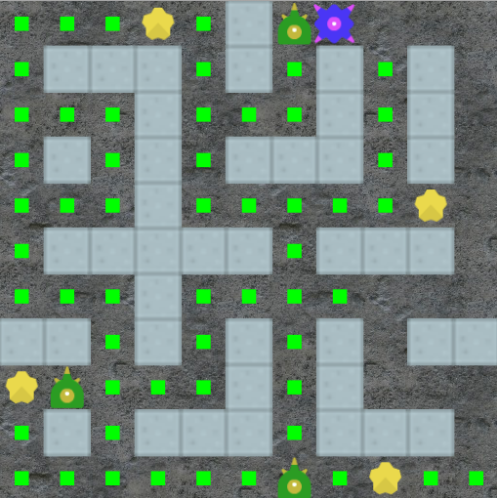
\includegraphics[scale=0.3]{abb/ss_chaser_gros}
        \caption{Chaser - unskaliert.}
        \label{fig:pic_chaserGros}
    \end{minipage}
    %\hfill
    \begin{minipage}{0.45\linewidth}
        \centering
        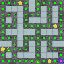
\includegraphics[scale=2.35]{abb/ss_chaser_klein}
        \caption{Chaser - herunterskaliert.}
        \label{fig:pic_chaserKlein}
    \end{minipage}
    %\caption{Chaser Environment - links unskaliert, rechts skaliert}
\end{figure}


Folgend wird das gewählte Spiel Chaser für die Experimente vorgestellt. Ein Bild des Spiels kann Abbildung \ref{fig:pic_chaserGros} entnommen werden. Ein Blick auf den Input des Agenten bietet die Abbildung \ref{fig:pic_chaserKlein}. Dieser ist auf $64 * 64$ Pixel herunter skaliert. 
Das Spiel Chaser ist von dem Atari-Klassier \dq Ms. Pac-Man\dq{} inspiriert. Der Agent spielt den \emph{Jäger}. Ziel des Jägers ist es, alle auf der Karte befindlichen grünen Orbs einzusammeln. Bei Erfüllung des Ziels bekommt der Agent einen hohen extra Reward von 10 Punkten. Zum Vergleich: ein normaler grüner Orb gibt nur einen Reward von 0.04. Unterdessen muss der Agent den drei Geistern ausweichen, die sich im Spiel befinden.

Die Geister können sich in vier verschiedenen States befinden. Diese werden folgend erläutert.
  \begin{itemize}
    	\item \emph{idle-State}: Dieser State ist ein Übergangsstate, in welchem die Geister auf dem Spielfeld erscheinen. Nach $t_1$ Sekunden wird der Geist automatisch in den tödlich-State überführt. Dieser State ist optisch durch ein eigenes Sprite differenziert. Geister in diesem State bewegen sich nicht und können dem Jäger noch nicht schade. 
  	\item \emph{tödlich-State}: Eine Berührung des Jägers mit einem Geist in diesem State beendet die Episode. Die Geister laufen in diesem State zufällig und ziellos. 
  	\item \emph{verletzlich-State}: Geister können vom Jäger in diesem State gefressen werden. Sammelt der Jäger einen großen Orb ein, überführt er die Geister damit in diesen State. Dieser State ist optisch durch ein eigenes Sprite differenziert. Dieser State führt nach $t_2$ Sekunden wieder in den tödlich-State, wenn der Geist nicht gefressen wird.
  	\item \emph{killing-State}: Ist ein Geist zwei oder weniger Felder vom Jäger entfernt, so wird der Geist in diesen State überführt. In diesem State läuft der Geist nicht mehr in zufällige Ricthungen, sondern zielstrebig auf den Jäger zu. 
  \end{itemize}

Der Action Space des Agenten ist diskret und beläuft sich auf 15 Aktionen. Dem Agenten steht dabei die folgende Menge an Actions zur Verfügung: \\ \newline
$ ~ M = \{ \leftarrow, \uparrow, \rightarrow, \downarrow,  \leftarrow + \uparrow, ~ \uparrow + \rightarrow, ~ \rightarrow + \downarrow, ~\downarrow + \leftarrow, ~'stehen~bleiben', W, A, S, D, Q, E \}$. \newline


Diese beinhalten 'stehen bleiben' und 'laufen' in vier Richtungen, mit der Option eine Richtungstaste mit einer daneben liegenden zu kombinieren ($ \leftarrow + \uparrow, ~ \uparrow + \rightarrow, ~ \rightarrow + \downarrow, ~\downarrow + \leftarrow $). Die Kombination aus zwei Richtungstasten führt jeweils zu einer eigenen Action. Bspw. führen die Richtungen 'hoch' $\uparrow$ und 'links' $\leftarrow$ zusammen zur Action 'hoch-links' $\uparrow \leftarrow$. Bewegt sich der Agent bspw. aktuell nach oben und die Action 'hoch-links' ($\leftarrow \uparrow$) wird ausgeführt, so läuft der Agent so lange 'hoch', bis sich die nächste Möglichkeit nach links zu laufen ergibt. Dann läuft er automatisch 'links'. Der Action Space beinhaltet nicht nur die vier Richtungstasten und die Kombinationen nebeneinander liegender Richtungen, sondern auch die Tasten W, A, S, D, Q und E. Hierbei sind die Tasten W, A, S und D gleich belegt wie die Tasten $\uparrow, \leftarrow, \downarrow und \rightarrow$ (in der selben Reihenfolge). Die Tasten Q und E sind gleich belegt wie die Kombinationen $\leftarrow + \uparrow, ~ \uparrow + \rightarrow$. Durch die Redundanz im Action Space mit den Buchstaben-Tasten, lässt sich die Anzahl der möglichen Aktionen von 15 auf 9 reduzieren. Dabei werden die Tasten W, A, S, D, Q und E deaktiviert. Aus Gründen der Vergleichbarkeit zu anderen Arbeiten, wird in dieser Arbeit durchweg mit 15 Actions gearbeitet.


Das Spiel kann in drei verschiedenen Modi gespielt werden. Diese States sind: Easy, Hard und Exploration

\begin{center}
 \begin{table}[htb!]
 \begin{center}
  \begin{tabular}{ l c c c c }
    \hline
     & Easy & Hard & Exploration \\ \hline \hline
     totaler Orb Reward & 0,04 & -1,04 & 1,04 \\ \hline
     extra Orb Reward & 0 & -1 & 1 \\ \hline
     Fertigstellungsbonus & 10 & 10 & 10 \\ \hline
     Spielfeldgröße & 11x11 & 13x13 & 19x19 \\ \hline
    \hline
    %\multicolumn{2}{|c|}{Info in einer Zelle} \\
    %\hline
  \end{tabular}
  \caption{Übersicht über die unterschiedlichen Reward-Settings. Vergabe der Rewards für Orbs ist abhängig vom gewählten Modus.}
  \label{tab:tab_reward_Modi}
  \end{center}
 \end{table}
\end{center} 

Diese unterscheiden sich in der Größe des Spielfelds und im Reward-Systems. Die Vergabe der Rewards durch das Environment ist abhängig vom gewählten Modus und lässt sich in Tabelle \ref{tab:tab_reward_Modi} ablesen. Diese Arbeit verwendet ausschließlich den Modus \emph{Easy}. In jedem Modus sind drei Gegner auf dem Spielfeld. Diese erscheinen jedes Spiel an einer zufälligen Position in unterschiedlichen Quadranten des Spielfeldes. Das Fressen eines Geistes bringt keinen Reward, ebensowenig wie das Gefressen werden.

Der State Space des Environments ist insofern variabel, dass die PCG nicht immer Level mit der selben Anzahl an freien Feldern hervorbringt. Bezogen auf die möglichen Pixel-Verteilungen ergibt sich ein theoretischer State Space von 68,7 Mrd. \footnote{256 Farben pro Farbkanal, drei Farbkanäle, bei einer Bildgröße von 64 auf 64 Pixel. ($256^3 * 64 * 64 = 68.719.476.736$)} möglichen States. Jedoch ist diese Zahl nicht die tatsächliche Größe des State Spaces, da die Berechnung der 68,7 Mrd. auf der Annahme stützt, dass jedes Pixel jede mögliche Farbe annehmen kann. Durch den Algorithmus der Level-Erstellung und die Verwendung von Sprites wird die Zahl deutlich reduziert. 

Das Layout des Levels wird mit prozeduraler Generierung erstellt. Mit Hilfe des Kruskal Algorithmus \cite{kruskal1956shortest}~[S.48-50] wird ein Spanning Tree über das Spielfeld gelegt, welcher alle Felder miteinander verbindet. Daraufhin werden so lange Wände entfernt, bis keine toten Enden mehr unter den Pfaden sind. Das Environment ist deterministisch, bis auf die Geister im tödlich-State. In diesem State bewegen sich die Geister zufällig durch das Level. Formal gesehen entspricht das Environment somit einem POMDP \cite{astrom1965optimal}.

Aufgrund des hohen Rewards von $10$ für den letzten eingesammelten Orb, kann davon ausgegangen werden, dass ein Agent mit einem durchschnittlichen Reward $ \geq 10$ in der Evaluation erfolgreich besteht. Erreicht ein Agent in der Evaluation eines Checkpoint bspw. einen durchschnittlichen Reward $\geq 10$, so kann man sagen, dass der Agent in der Evaluation besteht. 

%\subsubsection{Hintergrund}\label{absch_RL_hintergrund}




\newpage